\documentclass[11pt,a4paper]{article}
\usepackage[margin=23mm,top=22mm,bottom=23mm,headheight=14pt]{geometry}
\usepackage{fontspec}
\setmainfont{P052-Roman.otf}[BoldFont=P052-Bold.otf,ItalicFont=P052-Italic.otf,BoldItalicFont=P052-BoldItalic.otf]
\setsansfont{NimbusSans-Regular.otf}[BoldFont=NimbusSans-Bold.otf,ItalicFont=NimbusSans-Italic.otf,BoldItalicFont=NimbusSans-BoldItalic.otf]
\setmonofont[Scale=0.83]{Latin Modern Mono}
\usepackage{microtype,amsmath,amssymb,graphicx,booktabs,array,longtable,tabularx}
\usepackage[table]{xcolor}
\usepackage{titlesec,enumitem,fancyhdr,xurl,float,caption,needspace}
\usepackage[most]{tcolorbox}
\usepackage[numbers,sort&compress]{natbib}
\usepackage{hyperref}
\definecolor{AlphaPurple}{HTML}{45216B}
\definecolor{AlphaInk}{HTML}{22182D}
\definecolor{AlphaLilac}{HTML}{F3EEF8}
\definecolor{AlphaTeal}{HTML}{167C80}
\definecolor{AlphaGray}{HTML}{625A69}
\hypersetup{colorlinks=true,linkcolor=AlphaPurple,citecolor=AlphaPurple,urlcolor=AlphaPurple,
 pdftitle={The Economy of Verified Capability},pdfauthor={Vincent Boucher, MONTREAL.AI},
 pdfsubject={Game-Theoretic Investment in a Growing Validated Skills Graph}}
\urlstyle{tt}
\titleformat{\section}{\Large\sffamily\bfseries\color{AlphaPurple}}{\thesection}{0.7em}{}
\titleformat{\subsection}{\large\sffamily\bfseries\color{AlphaInk}}{\thesubsection}{0.7em}{}
\titleformat{\subsubsection}{\normalsize\sffamily\bfseries\color{AlphaInk}}{\thesubsubsection}{0.7em}{}
\titlespacing*{\section}{0pt}{2.1ex plus .5ex}{1ex}
\titlespacing*{\subsection}{0pt}{1.6ex plus .3ex}{.5ex}
\setlength{\parskip}{4pt}
\setlength{\parindent}{0pt}
\setlength{\emergencystretch}{2em}
\setlist{nosep,leftmargin=1.5em,topsep=3pt}
\captionsetup{font=small,labelfont={bf,sf},textfont=normalfont,labelsep=period}
\newcolumntype{Y}{>{\raggedright\arraybackslash}X}
\newcolumntype{L}[1]{>{\raggedright\arraybackslash}p{#1}}
\newcommand{\code}[1]{\nolinkurl{#1}}
\newcommand{\artifact}[1]{\nolinkurl{#1}}
\newcommand{\scopebox}[2]{\begin{tcolorbox}[colback=AlphaLilac,colframe=AlphaPurple,boxrule=.5pt,arc=1mm,left=2.5mm,right=2.5mm,top=1.8mm,bottom=1.8mm,title={#1},fonttitle=\sffamily\bfseries]#2\end{tcolorbox}}
\pagestyle{fancy}
\fancyhf{}
\fancyhead[L]{\small\sffamily\color{AlphaGray}AGI ALPHA FLYWHEEL}
\fancyhead[R]{\small\sffamily\color{AlphaGray}The Economy of Verified Capability}
\fancyfoot[L]{\footnotesize\sffamily\color{AlphaGray}Research edition \ReportDate}
\fancyfoot[R]{\small\sffamily\thepage}
\renewcommand{\headrulewidth}{.3pt}
\renewcommand{\footrulewidth}{0pt}
\newcommand{\ReportDate}{26 October 2026}
\newcommand{\ReportState}{Completed bounded research; review edition}
\newcommand{\RegistryOneoff}{\$88.50}
\newcommand{\GraphOneoff}{\$90.50}
\newcommand{\RegistryWeekly}{\$0.25}
\newcommand{\GraphWeekly}{\$0.40}
\newcommand{\AbstractProductionResult}{All 72 of 72 packets were accepted with equivalent decisions. Mean primary wall times were graph 1.6659 s, registry 1.6790 s, native incumbent 1.5976 s and direct conventional 1.3846 s; graph selection itself was slower than registry selection.}
\newcommand{\FrenchResult}{Les 72 dossiers ont été acceptés selon le même critère technique. Dans 1 152 mondes conditionnels, 24 tentatives du graphe sont financées par les ressources simulées, mais 0 satisfait le critère complet d'investissement. Les 288 cas à coûts inconnus restent indéterminés.}
\newcommand{\ProductionEquivalence}{True}
\newcommand{\AbstractMarketResult}{The 1,152 paired modeled worlds produced 0 qualifying graph second investments and 0 qualifying registry investments; 24 graph attempts were funded from modeled generated resources.}


\begin{document}
\thispagestyle{empty}
{\sffamily\bfseries\color{AlphaPurple}\large AGI ALPHA FLYWHEEL\hfill SUCCESSOR $\Omega$\par}
\vspace{10mm}
{\sffamily\bfseries\color{AlphaInk}\fontsize{29}{33}\selectfont The Economy of\\Verified Capability\par}
\vspace{4mm}
{\sffamily\color{AlphaPurple}\Large Game-Theoretic Investment in a\\Growing Validated Skills Graph\par}
\vspace{6mm}
{\large Vincent Boucher}\hfill{\sffamily MONTREAL.AI}\\
{\small\color{AlphaGray}\ReportDate\quad\textbullet\quad Additive research edition\quad\textbullet\quad\ReportState}
\vspace{5mm}

\textbf{Abstract.}
Reusable capabilities create value when they improve accepted useful work enough to cover their discovery, construction, validation and upkeep. A growing graph and a valid inclusion proof do not establish that return. We add a scoped capability layer to the existing AGI ALPHA native SUCCESSOR Workbench without changing Jobs roles, contracts, validation or settlement. The implementation separates execution observations, technical admission and economic admission; distinguishes agent-identity attestation from graph-root permission; and preserves typed commitments, authorization history and current-use blocking conditions. A clearly labeled fixture tests exact-node authority rules. Live identity enforcement is \textbf{NOT RUN}.

The offering is a source-bound dependency decision packet for a declared native Python environment. Four workflows evaluate 15 previously unexecuted, correlated pairwise dependency compositions and three separately designated requirement stresses. The graph and a strong cached registry receive identical skills, evidence, authority checks, freshness rules and ordinary caches. A direct conventional alternative tests the cost of the native integration constraint. \AbstractProductionResult\ Measured production effects feed the unchanged canonical monetary ledger and inherited heterogeneous buyer/competitor simulator. \AbstractMarketResult\ Complete actual authoring, attention and future maintenance costs remain unknown. The evidence supports bounded implementation and within-model conclusions; it does not establish customer demand, live ENS authentication, deployed graph authority, realized commercial success, equilibrium or self-acceleration.

\scopebox{Evidence boundary}{\small
\textbf{Executed:} native/direct production, metadata verification, scoped fixture admission, graph/registry selection and frozen market simulation.\quad
\textbf{Modeled:} demand, prices, competition, labor rates, investments, collections and surplus.\quad
\textbf{Unobserved:} customer acceptance and human savings.\quad
\textbf{Actual customer collections:} zero.}

\vfill
{\footnotesize\color{AlphaGray}Assistant-assisted research and implementation. Separate implementation and review agents worked in the same session; this is not external peer review. The original foundations and prior negative research editions remain intact. The accompanying source/evidence package is the reproducible record.}
\newpage

\section*{Résumé}
Une compétence réutilisable mérite un investissement lorsqu'elle améliore des résultats utiles et acceptés suffisamment pour couvrir sa découverte, sa construction, sa validation et son entretien. L'augmentation du nombre de nœuds ou de preuves d'inclusion ne démontre pas cette valeur. Cette étude ajoute au système AGI ALPHA existant un graphe de compétences exécutables, versionnées et limitées à un périmètre vérifié. Les rôles de validation Jobs, les contrats et le règlement restent inchangés.

L'offre étudiée est un dossier de décision sur la cohérence des métadonnées d'un ensemble exact de dépendances Python. Le dossier comprend les sources, les journaux et les témoins de conflit nécessaires à l'examen. Nous comparons le processus natif, un registre consultable doté d'une recette mise en cache, le graphe et une solution conventionnelle directe. Les deux couches de réutilisation ont les mêmes compétences et les mêmes éléments de preuve. Quinze compositions nouvelles de sources historiques constituent la cohorte principale; trois changements d'exigences servent de tests de résistance séparés. Ces cas partagent des composants et ne constituent donc pas quinze écosystèmes indépendants.

L'autorisation de produire une attestation de compétence est distincte de l'autorisation d'engager une racine du graphe. Les identités et les permissions sont des \emph{fixtures de recherche explicites}; la vérification d'identité en conditions réelles est \textbf{NON EXÉCUTÉE}. Une preuve de Merkle engage un enregistrement précis, sans démontrer la vérité, la compétence du signataire ou la rentabilité. Les coûts mesurés alimentent une simulation de clients et de concurrents. Les achats et le surplus de cette simulation ne sont jamais présentés comme des recettes réelles. \FrenchResult\ Les coûts complets réels restent inconnus et l'investissement nul demeure une décision admissible.

\section{Research question and inherited evidence}
\label{sec:question}
The proposed flywheel links useful work, profitable delivery, worthwhile investment, validated reusable capability, improved fresh work and resources for another investment. Each arrow is an empirical obligation. A capability may execute correctly yet be too expensive to adopt. A firm may earn simulated operating surplus yet have no improvement worth funding. A proof can preserve a claim accurately while the claim is wrong. This study asks whether adding evidence-backed relationships changes production enough to repay the additional layer.

The research starts from an observed internal need in the public Alpha project: maintainers must assess exact dependency changes against declared native requirements. Commercial recurring demand for that service is modeled, not observed. The graph itself is infrastructure for the offering. No independent evidence here establishes a market for purchasing graphs, attestations or Merkle proofs as products.

The original project foundations remain the integration context: AGI-Alpha-Agent-v0, AGI-Fleet-Linux, AGIJobsv0 and AGIJobManager \citep{alpha,fleet,jobs,jobmanager}. Coordination follows issue 4850 \citep{issue4850}. The executed native closure comes from the existing SUCCESSOR Workbench, with upstream identities retained. Its historical imports, state transitions and authority limitations are preserved. The additive sidecar does not introduce a competing scheduler, accounting system, native identity service or settlement path.

\subsection{What this edition inherits}
The prior research program contains a primary negative result, conditional deployment gains, a conventional-builder tie and an unsuccessful second-investment search. These are different results at different cost boundaries; none is replaced by the current experiment. Prospective deployment value can be positive while total historical research costs remain unrecovered. Equal conventional performance prevents attributing an effect to a distinctive intelligence architecture. The absence of a worthwhile second investment remains evidence against an unrestricted self-financing improvement claim. Appendix~\ref{app:heritage} records the preserved sources and their result boundaries.

We retain the PR 4940 production/verification components and canonical economic sources byte for byte \citep{priorsecond}. The new strong incumbent is the previously retained native workflow. Registry and graph compositions wrap the same available components and evidence. We do not give the graph an improved underlying producer while assigning that improvement to its topology.

\subsection{Contribution and disconfirming condition}
The contribution is an implemented, falsifiable layer with a scoped authority model, typed commitment history, current-use gates, a matched registry comparator, complete execution measurements and a finite economic test. The structural hypothesis is that preserving executable relations between requirements, methods, evidence and accepted compositions can reduce repeated selection work or prevent invalid reuse before expensive delivery. The observed engineering burden is repeated reconstruction of these relationships and the need to distinguish current admissibility from a historically accepted record. Its labor cost has not been measured.

The hypothesis is disconfirmed for this offering if a strong ordinary registry with a reusable validated recipe obtains the same accepted outcomes at equal or lower complete cost, or if any graph saving fails to recover construction and upkeep. A safety gate that both B and C possess is not evidence for graph topology. A successful refusal is useful control behavior but does not create a customer order, a paid job or an investment return.

\section{A useful, executable offering}
\label{sec:offering}
The customer-facing output is a complete dependency decision packet. It answers a narrow question: does this exact wheel-only lock satisfy the declared project roots, selected extras, Python range and all active wheel-metadata constraints in the specified environment? A useful outcome can be a substantiated conflict. The buyer can hold an incompatible proposal, inspect a concrete witness, or proceed to further application qualification after a consistent metadata result. Metadata consistency does not establish installation, runtime behavior, security or release readiness.

The implemented pipeline binds the job, requirements, project metadata, selected wheel identities, environment and source closure. It invokes ordinary pip using the existing wheel cache and retains stdout, stderr and the raw report. The independent deterministic verifier re-parses wheel METADATA/WHEEL information, evaluates markers and recursive extras, checks exact requirements, and reconciles the producer's decision. The final artifact contains an evidence inventory, English/French report and ZIP package. A receipt is accepted only if the actual result and supporting evidence pass the frozen acceptance contract.

\subsection{Mission triggers and acceptance}
The semantic mission key includes active lock requirements and hashes, selected wheel identities, declared roots/extras/Python range and environment. An alias, path move, prose edit or comment-only change does not create another substantive mission. A changed requirement, dependency or environment does. This distinction prevents unchanged requests from inflating completed-work counts.

Three outcomes are possible: a complete \code{CONSISTENT} packet; a complete \code{CONFLICT} packet with substantiated witnesses; or an unaccepted \code{INCOMPLETE}/refusal with retained evidence. The unchanged native pack remains \code{HOLD} and \code{UNAUTHENTICATED_HISTORICAL_IMPORT}, with empty active proof/authority fields. A new fixture-only graph admission does not lift that native restriction.

Fresh composition results are evaluated independently. Two individually accepted dependency substitutions can interact; one component's evidence cannot authorize the combined lock. Likewise, a sequence of technically valid methods requires evidence for the combined workflow, including its source-bound implementation, required members and outputs. This implements the scoped reuse rule in PROOF LOOPS rather than a closure assumption that every combination of valid parts is valid \citep[§§11,14, pp.~5,7]{proofloops}.

\section{Executable assets and the validated graph}
\label{sec:graph}
The small catalogue contains four scoped methods: lock preflight, metadata verification, native Workbench execution and decision delivery. Each skill record binds its identifier and version to implementation and dependency digests; supported inputs, outputs and preconditions; limits and known failures; refusal and rollback behavior; evidence; rights; costs; and lifecycle state. A skill is a reproducible procedure with a declared use envelope. An attractive natural-language description alone is not a capability.

Execution observations describe what happened. Technical admission states that the evidence satisfies a particular policy within scope. Economic admission asks whether an available asset improves the chosen offering enough to cover its complete incremental cost. These records are deliberately distinct. Initial catalogue technical admissions remain economically unassessed until production and market analysis are available. No inclusion proof grants economic admission.

\subsection{Relationships and combined-workflow evidence}
The typed relationship layer can express dependency, compatibility, composition, substitution and conflict. In this catalogue, selection uses explicit dependency and composition relations associated with the exact scope and a combined-workflow dossier. Record fields identify both endpoints and versions, the relation's policy and evidence, and applicable conditions. A relation carries a claim that must be checked; it is not true because its edge exists.

The final selector verifies the committed inventory, the displayed descriptor bindings, exact required dependencies, composition membership and lifecycle state before allowing influence. It obtains revocations and supersessions from the committed records. Missing evidence, stale authority, inconsistent dependencies or an unvalidated composition block current selection. The selector owns an immutable copy of its input frame, preventing a resolver callback from changing a previously checked catalogue or caller context during the decision.

The registry comparator contains the same relationship dossiers. Its output index and cached independently validated recipe directly identify a composition, with ordinary dossier lookup and admissibility checks. The graph traverses typed adjacency to obtain the same required sequence. Both may retain assets and caches. Replacing traversal with the registry recipe is the primary structural ablation; unequal evidence access would confound it.

\subsection{History, repair and retirement}
Following PROOF LOOPS, current reuse requires admission, scope match, freshness and absence of a blocking condition \citep[§14, p.~7]{proofloops}:
\begin{equation}
\operatorname{Reuse}(s,m,t)=\operatorname{Admitted}(s)\land
\operatorname{ScopeMatch}(s,m)\land\operatorname{Fresh}(s,t)\land
\neg\operatorname{Blocked}(s,m,t).
\end{equation}
An expired or revoked skill can remain a historically included record while losing future influence. Supersession points to a successor rather than erasing the former version. A source change creates a revalidation obligation. Repair is new work with its own evidence and cost; silently adjusting a frozen experiment is not repair. Fallback returns to the existing native workflow where allowed by the offering, otherwise the system refuses.

The graph has only four skills and two construction epochs in this study. Growth means an actual addition from an incomplete capability set to the complete tested composition. The experiment does not estimate search complexity or general scaling in large, heterogeneous graphs. Its value lies in testing the semantics and the complete cost of a plausible small deployment.

\section{Identity, authority and commitment are separate}
\label{sec:authority}
The user-required graph attestation policy is additional to the Merkle paper's root-writer rule. Only an eligible authenticated agent identity may authorize this graph's validated-skill admission. Existing Jobs validators and their \code{*.club.agi.eth} requirements remain unchanged. Job results and reviews can support a dossier, but cannot independently authorize admission to this new graph.

Two operation names prevent permission conflation: \code{ISSUE_SKILL_ATTESTATION} and \code{COMMIT_GRAPH_ROOT}. An attester without a root grant cannot write a root; a root writer without an attestation grant cannot validate a skill. The Merkle paper describes direct \code{label.agent.agi.eth} root authority in §12, printed p.~12, but does not establish this exclusive attestation policy \citep{merkle}.

\subsection{Exact-node authority and fixture boundary}
The research policy supports a conservative direct ASCII single label under \code{agent.agi.eth}. It rejects deeper subnames, club identities and other namespaces. This is not a full ENSIP-15 implementation \citep{ensnames}. An ENS-looking string, address resolution record or reverse name is insufficient. A production adapter would verify the exact node, chain, registry version/code, block state and actual signature, then resolve the applicable current authority.

The bounded resolver models unwrapped exact-node ownership, a wrapped name's current holder, full-control operators and operation-scoped delegation. Registry ownership and \code{isApprovedForAll} provide distinct authority inputs \citep{ensregistry}. When a name is wrapped, the wrapper holder and full-control approval must be checked. The NameWrapper's per-name \code{approve}/\code{getApproved} renewal permission is not general control; this experiment explicitly refuses it as an attestation or root grant \citep{enswrapper}. Expiry and changed authority epochs block current use \citep{ensexpiry}. Unknown registry or authority models fail closed, including unqualified assumptions about ENSv2 \citep{ensv2}.

The implementation creates no credentials and performs no transactions. Its simulated envelope verifier is labeled \code{FIXTURE_NOT_CRYPTOGRAPHIC}. The return value always discloses \code{cryptographicAuthentication:false}; live mode fails closed with \code{NOT_RUN}. Fixture success demonstrates the policy logic under declared authority states. It does not authenticate control of an actual ENS name. A future live adapter would separately require an EOA signature recovery or ERC-1271 contract check, a supported registry-state verification path and an operational trust policy. EIP-712 alone does not provide replay protection, while ERC-1271 validity can depend on state \citep{eip712,eip1271}.

\subsection{Context binding and historical validity}
An attestation binds the exact skill/version, implementation and dependencies, evidence, scope, environment, policy, reuse rights, issue and expiry times, nonce, operation, graph namespace, chain, registry and authority snapshot. A changed digest is a different claim. Admission replay checks use a consumed nonce set; legitimate read-only reuse of the same admitted attestation does not consume another admission. Historical validity is evaluated against the bound issuance state. Current reuse additionally requires current authority, unexpired context and absence of revocation/supersession. A transfer therefore need not falsify a historical attestation, but can invalidate its present permission under this conservative policy.

A root write independently binds expected epoch and predecessor through compare-and-swap checks, plus the exact forest roots/counts, policy, context and writer state. Admission and lifecycle verification are required separately. The root authorizer does not infer evidence truth from the writer's permission.

\subsection{Typed commitments and whole-inventory checks}
The implementation follows the Merkle paper's separation of capability, evidence, commitment and authority \citep[§§1,5, pp.~2--3,5]{merkle}. Its nine typed classes are \code{skill}, \code{edge}, \code{evidence}, \code{proofbundle}, \code{policy}, \code{attestation}, \code{revocation}, \code{supersession} and \code{metadata}. Costs, admissions and successor descriptors are represented within appropriately typed records, not silently substituted for the paper's classes.

This research uses a declared SHA-256 profile, safe-integer canonical JSON, NFC strings and domain-separated leaves. It is not presented as wire-compatible with every architecture in the source paper. A leaf includes its type/schema; pairs are sorted, odd leaves duplicated, duplicates refused and empty roots deterministic. Epochs commit class roots and counts, predecessor, namespace and policy. Inclusion establishes membership of exact committed bytes. It cannot prove record truth, signer's competence, completeness of an arbitrary caller-supplied inventory, or economic usefulness. The selector therefore reconstructs the full supplied forest and matches committed roots/counts before applying lifecycle controls. One valid inclusion proof must not conceal an omitted revocation.

\section{Frozen production design}
\label{sec:design}
Candidate selection, acceptance, cohort construction, arm order and source/input identities are frozen before any fresh production outcome. Development uses the inherited unchanged lock; its repeated baseline is not counted as a fresh result. The primary cohort contains all 15 lexicographically ordered pairs drawn from six archived predecessor substitutions: cryptography, eth-account, prometheus-client, pydantic-settings, PyYAML and uvicorn. The pairing creates previously unexecuted combined questions while preserving unsuccessful tuples.

These questions are correlated and reuse historical public artifacts. They are not 15 independent ecosystems, contemporary new releases, prospectively sampled customer orders or a broad benchmark. Three separate root changes test a cryptography major requirement, removal of a selected chain extra and an incompatible Python minimum. The stresses assess defined boundary behavior and do not enter the primary economic effect calibration.

\begin{table}[htbp]
\caption{Matched workflows and attribution boundary.}
\label{tab:arms}
\small
\begin{tabularx}{\linewidth}{L{10mm}L{37mm}Y}
\toprule Arm & Workflow & Resources and acceptance \\
\midrule
A & Native incumbent & Existing native Workbench, ordinary pip/hash caches, independent metadata verification and common delivery package. \\
B & Cached registry & Same skills, evidence, typed integrity, agent fixture authority and freshness policy; an output-indexed validated recipe selects the composition. \\
C & Validated graph & Same B inputs and gates; explicit typed adjacency traversal selects required methods and their composition. \\
D & Direct conventional & Existing direct producer, identical metadata acceptance and delivery package; omits the native history integration requirement. \\
\bottomrule
\end{tabularx}
\end{table}

All four arms run once per mission in frozen balanced interleaving: each arm appears four or five times in each of the four positions. The study reports finite-cohort paired elapsed and CPU differences. It does not mine repeated runs for significance, treat shared combinations as independent samples, or translate wall time into human attention. Failures remain in denominators. Any post-freeze correction would require a separate edition preserving the original results.

\subsection{Complete measurement and controls}
Measurement includes producer interpreter startup, waited subprocess descendants, actual ordinary pip, independent verification, native recording when applicable, report/ZIP packaging, selection, source checks and evidence custody. Shared initialization is allocated equally; selector construction belongs to its arm. Shared recurring overhead beyond per-mission rows is spread over all 18 fresh outcomes before the 15-primary mean is calculated. Cache confirmations are recorded separately with zero new jobs and zero new pip resolutions.

Technical controls cover source changes, missing evidence, invalid attestations, stale skills, ownership transfer, operation mismatch, nested names, revocation, supersession, conflicts, unvalidated composition, typed-record substitution and root-history replay. Production controls address malformed or nonfinite JSON, declared-source mismatch, input symlinks, stale certificates, unsupported builder decisions, mutated pip metadata, missing logs and path escape. Unsafe diagnostic ablations remove authority, freshness or compatibility gates to show their role. They are not eligible commercial workflows.

The creator--critic--verifier process accepts a critic's no-finding result. A claimed consequential defect must have a concrete reproduction and an independently checked consequence. Rejected designs, unsuccessful criticism, fixes and repeated validation consume resources. The preserved development review records document those costs and the limits of same-session review; they are not folded into a fictitious zero-cost initial capability.

\section{Complete economics and strategic markets}
\label{sec:economics}
The economic comparison has three boundaries. Marginal measured execution records elapsed/CPU/tool use for each accepted or failed attempt. Recurring modeled cost includes upkeep, storage and revalidation. Fully loaded incremental cost includes discovery, rejected candidates, construction, validation, identity verification, indexing, proof generation/checking, retrieval, composition, integration, researcher contribution, authoring tools and residual attention. Known quantities remain measured; unmetered actual authoring, inference, human attention and future upkeep remain unknown.

The new adapter maps every incremental monetary row into the existing canonical categories. It does not replace the economic ledger. Historical first-asset costs are counted once. New composition construction is distinguished from reuse of existing source. Completed research outside the modeled enterprise still reduces project-inclusive profit exactly once; it does not increase enterprise cash. Actual fully loaded cost is null rather than zero.

\subsection{Scenario costs and effect calibration}
Reference incremental allocations are generated directly from the frozen cost specification: \RegistryOneoff\ for B and \GraphOneoff\ for C, with \RegistryWeekly\ and \GraphWeekly\ weekly upkeep. Low and high profiles apply quarter/fourfold allocations with the simulator's per-row cent rounding. These are subjective scenario choices covering complete categories, not measured invoices or empirical lower/upper bounds. An actual-unknown profile preserves missing costs, including under a maintenance shock. Appendix~\ref{app:costs} gives every row.

Only matched accepted primary outcomes can earn a production saving. Let $c_a$ be inclusive mean CPU seconds per primary mission for arm $a$, and $p$ an assumed USD per core-hour tariff. The explicitly conditional conversion is
\begin{equation}
\Delta k_a(p)=\frac{(c_A-c_a)p}{3600}.
\end{equation}
The primary scenario uses $p=1$, with deterministic $0.1$ and $10$ sensitivities. Signed subcent effects are retained even when the inherited cent ledger rounds the marginal value to zero. No graph price premium, trust uplift, quality uplift or human/customer review saving is credited. Zero credit means unmeasured, not no human work. A separate break-even calculation reports the additional unmeasured human saving that would be required; it does not insert that saving into the production evidence or financial gate.

\subsection{Buyer behavior, competitors and limits}
The inherited repeated-procurement simulator has heterogeneous buyers with different needs, time values, budgets, error losses and quality beliefs. Offers include the enterprise, human providers, competing AI, conventional do-it-yourself software and deferral. Buyers can reject, delay, switch or leave. Their net utility for offer $j$ combines expected useful outcome value, price, review effort, delay, integration/switching cost and expected error loss:
\begin{equation}
U_{ij}=q_{ij}V_i-P_j-E_{ij}-D_{ij}-S_{ij}-(1-q_{ij})L_i.
\end{equation}
Positive-utility offers and doing nothing enter the frozen logit choice policy. Delayed outcome feedback changes quality beliefs. Competitors can adjust prices and make a modeled conventional automation response. Their response is an assumption in a behavioral simulation, not an actually built successor.

The finite campaign uses 52 weeks, 12 buyers, USD 1,000 initial seed and a USD 200 reserve. Reference price is USD 20, reference arrival probability is 0.5, and the favorable inherited zero-integration condition is explicit. Five stresses lower demand, remove demand, add buyer integration friction, raise maintenance or strengthen the competing AI. Two financing policies and four cost profiles, each using 24 new paired seeds, define 48 cells and 1,152 paired worlds. These worlds use common random inputs across A/B/C. Designed-cell frequencies are not probabilities of real commercial success. Calibration inserts measured CPU effects; simulation does not validate the demand, trust or behavioral assumptions. No equilibrium claim is made.

\subsection{The second investment and finite resources}
The second candidate is the actual registry/graph composition constructed, admitted under fixture policy and used on fresh work. Exact source/evidence identities bind the modeled asset to the executed one. A Boolean assertion that a prototype exists is insufficient. The inherited initial asset can be seed-funded. Further investment must use prior operating-generated resources after obligations and reserve; future benefits are not borrowed.

With cash $K$, unpaid obligations $O$, reserve $R$, collected operating receipts $C$, all accrued costs $E$ and the qualifying seed-paid opening-history cost $H$, the unchanged funding rule is
\begin{equation}
F=\max\{0,\min(K-O-R,\ C-E+H)\}.
\end{equation}
The $H$ adjustment distinguishes seed-financed historical research from operating-generation accounting; it does not refund history or create new capital. The adaptive policy pays discovery and can preserve reserves by retaining the incumbent. A fixed-checkpoint completed-research replay asks whether the already built research could have been financed. An affordable but uneconomic attempt remains an unqualified research attempt.

Financial qualification additionally requires technical admission, actual use, complete priced incremental costs, direct repayment and positive paired project-inclusive profit over the credible useful life. Alternatives include adopting the existing registry composition, adopting the graph composition, maintaining current records and retaining A. D is a real measured stronger production alternative; unknown complete adoption/integration costs prevent a global monetary ranking from being inferred merely from the native A/B/C market comparison.

\section{Results from the frozen evidence}
\label{sec:results}

The frozen production campaign completed 72 actual assessments of 18 substantive questions. 72/72 packets were accepted. Exact matched decisions were equivalent across all four arms. The primary cohort contained 9 conflict, 6 consistent outcomes per arm; the three designed stresses contained 2 conflict, 1 consistent. This denominator includes every registered question. Four unchanged-request checks were recorded as cache confirmations, with zero new completed jobs.

Primary inclusive mean complete wall times were A 1.5976 s, B 1.6790 s, C 1.6659 s and D 1.3846 s. C--B was -0.0131 s in elapsed time and -0.0189 s in CPU; C--A was +0.0683 s and +0.0708 s. C had higher complete elapsed time than B on 8/15 primary rows. These differences include experimental source-custody checks in every arm and therefore are not deployment-latency estimates. Process bootstrap wall time and final JSON serialization after sampling are explicitly outside the measurement boundary; authoring, human attention and future upkeep are not inferred from these times.

The source-bound graph and registry selected the same complete skill sequence. Any difference in relationship traversal is evaluated against the registry's legitimate cached recipe. Refusal controls and inclusion checks are reported separately; they do not add accepted fresh work. The direct alternative's primary C--D differences were +0.2813 s wall and +0.3048 s CPU. Native history is an integration constraint rather than a demonstrated customer premium.

Selection-only mean elapsed time was 0.015257 s for B and 0.016043 s for C; mean selection CPU was 0.017662 s and 0.018206 s. Thus the modest complete C--B timing difference is not evidence that adjacency traversal reduced selection cost. On the first primary selection both examined 4 relationship rows; B read 4 cached recipe members and C made 3 traversals. The graph did not remove a demonstrated repeated-reconstruction burden relative to the strong recipe in this small catalogue.


\begin{table}[htbp]
\caption{Executed production. Primary means include allocated initialization; the three designed stresses remain separate. Times are descriptive seconds on this host.}
\label{tab:production}
\small\begin{tabularx}{\linewidth}{Yrrrrr}
\toprule Arm & Accepted & Primary wall & Primary CPU & Stress wall & Stress CPU \\
\midrule
A native & 18/18 & 1.598 & 1.533 & 1.417 & 1.351 \\
B registry & 18/18 & 1.679 & 1.623 & 1.466 & 1.397 \\
C graph & 18/18 & 1.666 & 1.604 & 1.490 & 1.451 \\
D direct & 18/18 & 1.385 & 1.299 & 1.415 & 1.330 \\
\bottomrule
\end{tabularx}

\end{table}

\begin{figure}[htbp]
\centering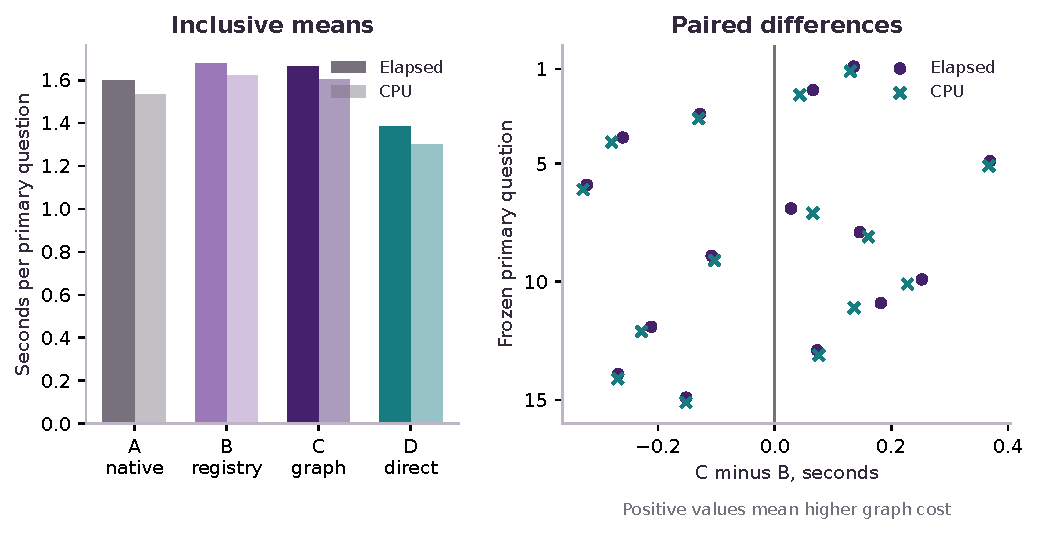
\includegraphics[width=\linewidth]{generated/production-comparison.pdf}
\caption{Paired complete primary production. A consistent decision and a substantiated conflict are both accepted scoped outcomes. The 15 rows share historical components; intervals are not population confidence bounds.}
\label{fig:production}
\end{figure}

\subsection{Native-market comparison and investments}

The fixed campaign completed 1,152 paired conditional worlds and 3,456 enterprise histories in 48 cells. Registry B had 24 operating-funded attempts and 0 complete financial-gate passes; graph C had 24 funded attempts and 0 passes. Funding and qualification are distinct. Across 864 priced C--A project differences, 863 were negative and 1 positive; 288 unknown-cost worlds remained unidentified. Of 36 priced cell means, 0 were positive. C--B project differences were negative in 864/864 priced worlds. These counts summarize a designed scenario grid rather than a random sample of markets.

No trust, price, quality or human-time benefit was assigned to graph proofs. The measured CPU effect was converted only at declared tariffs. The largest absolute graph microcent residual omitted by the cent-denominated ledger was USD 0.00049150 across a complete saved history; its sign is retained in the evidence. The complete-cost result includes completed outside research exactly once even when the enterprise declines construction, while preserving the enterprise's actual modeled cash balance. A negative project-inclusive difference can therefore coexist with a rational no-investment decision.


The one positive C--A realization is retained: the reference condition, low-cost completed-research replay, seed 9110, yields \$10.01. C receives \$40.00 more modeled collections and incurs \$29.99 additional accrued costs. B and C share the same changed buyer-choice path after the declared week-26 pause: buyer 1 chooses DIY instead of AI in weeks 26 and 32, then the enterprise instead of a human in weeks 47 and 49. Their accepted counts are 33 versus A's 31. C still trails B by \$1.50, has zero direct asset saving, a negative prospective investment forecast and no financial admission or direct repayment. This is descriptive analysis of saved traces, not a graph-specific causal finding or a new pause-only experiment. The exact path and arithmetic are retained in \artifact{review/positive-world-inspection.json}.


\begin{table}[htbp]
\caption{Reference market condition by financing policy and cost profile. Values are modeled USD, with paired C--A project-inclusive differences. Unknown complete costs remain unknown.}
\label{tab:market}
\small\begin{tabularx}{\linewidth}{YYrrrr}
\toprule Policy & Cost & C--A mean & 5th / 95th & Funded C & C gate \\
\midrule
Adaptive & Low & -22.63 & -22.63 / -22.63 & 0/24 & 0/24 \\
Adaptive & Reference & -90.50 & -90.50 / -90.50 & 0/24 & 0/24 \\
Adaptive & High & -362.00 & -362.00 / -362.00 & 0/24 & 0/24 \\
Adaptive & Unknown & \textit{unknown} & \textit{unknown} & 0/24 & 0/24 \\
Replay & Low & -26.97 & -57.63 / -10.86 & 6/24 & 0/24 \\
Replay & Reference & -93.68 & -115.43 / -90.50 & 4/24 & 0/24 \\
Replay & High & -362.00 & -362.00 / -362.00 & 0/24 & 0/24 \\
Replay & Unknown & \textit{unknown} & \textit{unknown} & 0/24 & 0/24 \\
\bottomrule
\end{tabularx}

\end{table}

\begin{figure}[htbp]
\centering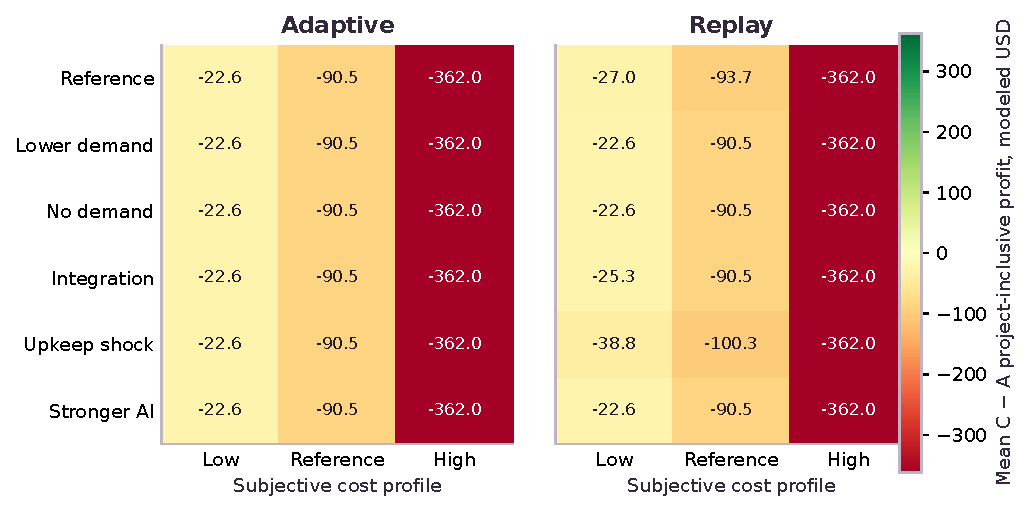
\includegraphics[width=\linewidth]{generated/market-regions.pdf}
\caption{Mean paired C--A project-inclusive profit by declared scenario. These are conditional within-model differences, not market probabilities. Unknown-cost cells are omitted from color arithmetic and retained in the tables.}
\label{fig:regions}
\end{figure}

\subsection{Reconciled resources and the direct alternative}

The predeclared reference-condition, reference-cost replay for seed 9101 ends with modeled C cash \$530.85, collections \$180.00, unpaid obligations \$0.00 and a \$200.00 reserve. At its first checkpoint, available operating-generated resources were \$0.00, against a complete graph one-off allocation of \$90.50. It made 0 modeled invocations of the source-bound graph composition and did not pass the complete financial gate. Its C--A project-inclusive difference was \$-90.50. The saved funding/expense/invoice records, rather than nominal ending cash alone, determine whether an attempt was financed.

Direct D is preserved as a real production alternative. Its matched CPU/elapsed means and tariff sensitivities are in \artifact{evidence/market-primary/effect-calibration.json}. The native continuation does not supply an independently calibrated D demand model or a complete D adoption-cost measurement, so a global adoption result against D remains unknown. Actual customer collections in every arm are zero.

\begin{figure}[htbp]
\centering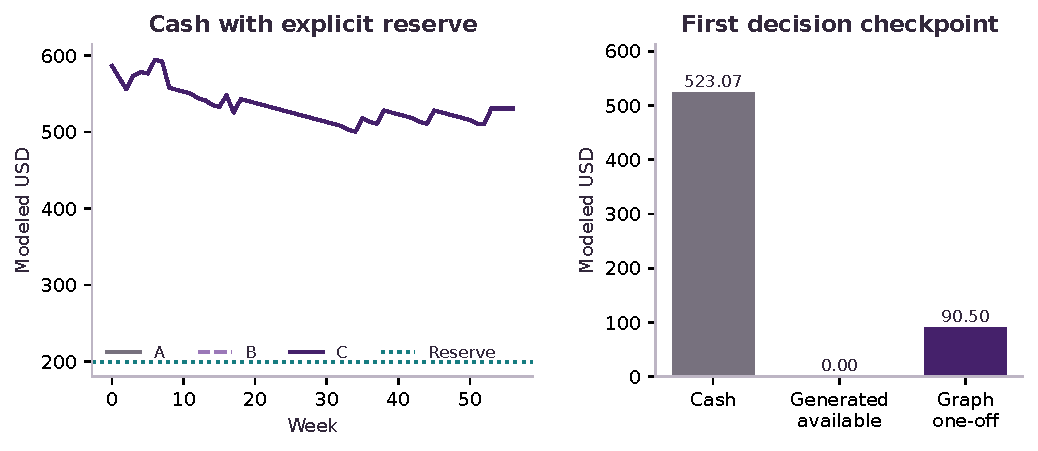
\includegraphics[width=.96\linewidth]{generated/cash-resources.pdf}
\caption{Reference-profile, reference-condition, seed 9101 resource histories. Every monetary quantity is simulated. Reserve and generated-resource constraints prevent unused seed cash from becoming an operating-funded reinvestment claim.}
\label{fig:cash}
\end{figure}

\section{What the controls establish}
\label{sec:controls}
The identity/commitment suite contains 80 passing direct tests after the R7 ownership repair: 54 authority and 26 commitment checks. An independent Python computation reproduces typed leaves, an odd-node Merkle root and the complete epoch commitment. This cross-language check verifies the declared serialization/hash profile; it does not certify a production cryptographic protocol or ENS registry adapter. Appendix~\ref{app:review} records the separate review receipts and preserved earlier failures.

One substantive preconfirmation defect concerned mutable caller state. A malicious or simply stateful resolver callback could previously alter the expected epoch before root compare-and-swap, or clear a shallow-copied revocation array before current-use evaluation. The corrected authorizers canonically copy and freeze their contexts before any callback. Fixture constructors likewise own payload/options before resolving authority state. The tests verify that callback mutation cannot repair an invalid original context or change an owned signed envelope.

Another review concern was the distinction between custody and evidence truth. An imported certificate could preserve consistent byte links while repeating an unsubstantiated builder verdict. The review constructed a mutated copy and compared custody checking with a fresh independent verifier; source admission was strengthened before freeze to require actual revalidation. Whole-forest reconstruction similarly prevents an inventory that supplies only valid inclusion paths from hiding lifecycle records. The original failing probes and source identities remain available. These repairs were preconfirmation engineering, not evidence of improved fresh market outcomes.

Common authority, provenance and freshness checks can prevent inappropriate reuse in both B and C. Their safety value must be distinguished from a topological production advantage. Diagnostic omission of a gate can demonstrate why that gate is required, but it does not make an intentionally unsafe comparator a competitive offering. Negative controls are therefore reported apart from accepted mission counts and economic calibration.

\section{Interpretation, limitations and deployment decision}
\label{sec:limits}
The implemented graph did not earn a justified second-investment result under the frozen financial gate. Technical admission, fresh use and a valid commitment chain were insufficient. The appropriate within-model action is to retain the strongest suitable incumbent or adopt a simpler existing method when its complete costs justify doing so; the actual all-in economic admission remains unknown because unmetered research and attention costs have not become measured invoices. A graph may still be maintained as research infrastructure, but that choice must carry its costs rather than be called commercial self-financing.


Several limitations constrain any stronger interpretation. The graph is deliberately tiny, its relation types are sparse and the offering narrow. A larger catalogue with changing dependencies could alter retrieval costs, but that is a future empirical claim. The 15 fresh primary questions are correlated combinations of archived substitutions. One interleaved run per arm measures this finite execution, with host noise and caching effects; it does not establish a general latency distribution. The verifier supports wheel metadata in the exact native environment and does not qualify installed applications.

The live identity boundary is equally material. Simulated authority states can exercise owner, wrapper, delegation, expiry and transfer rules, but do not prove an eligible current ENS signer. The inspected foundation repository contains a local reference loop and historical contract atlas; source inspection alone does not prove current live graph deployment. The paper's nine-class research forest and SHA-256 canonicalization are declared implementation choices, not a claim of universal V107 compatibility or M0--M9 conformance \citep[§§18--23, pp.~15--18]{merkle}.

Human attention, actual authoring inference, future maintenance, customer acceptance and willingness to pay remain unobserved. Scenario costs cannot make those actual quantities known. CPU arithmetic is useful because it keeps a small machine effect visible, but a subcent effect does not establish a labor saving. No token price, speculative appreciation or automatic utility premium enters the analysis. Applicable \$AGIALPHA utility is architectural context; no token transaction, financing or valuation is assumed.

The contribution does not demonstrate self-acceleration. That would require evidence that identifying, constructing and validating worthwhile improvements itself becomes more effective, with the additional process costs paid. More admitted records, consecutive root hashes or simulated adaptation do not satisfy that condition. A technically successful implementation with an unfavorable economic test is a meaningful result: it identifies what the added layer must improve before it deserves deployment.

\section*{Reproducibility, data and authorship}
All original papers, source snapshots, source/version manifests, frozen protocols, measured production packets, monetary ledgers and review records are retained in the companion \citep{companion}. The paper's tables, figures and numeric prose are generated from \artifact{evidence/production-summary.json}, \artifact{evidence/market-primary/} and the frozen cost specification. The build refuses missing final results and writes an input/output hash receipt. Its figures use standard vector output. Exact reproduction commands and expected boundaries appear in Appendix~\ref{app:reproduce}.

Vincent Boucher is the named author for this AGI ALPHA contribution. Research, implementation, testing and manuscript preparation were assistant-assisted. Reviewers were separate agents in the same working session, with shared source access and no organizational independence. There was no external peer review, paid pilot, customer outreach, credential creation, financial transaction or deployed-contract change. Publication/release status must be taken from the actual coordination record; a local PDF does not establish a public release.

\clearpage
\appendix
\small
\section{Evidence ladder and foundational mapping}
\label{app:ladder}
\begin{longtable}{L{31mm}L{51mm}L{67mm}}
\caption{Each evidentiary level requires a distinct result.}\\
\toprule Level & Evidence in this study & What does not follow \\
\midrule\endfirsthead
\toprule Level & Evidence in this study & What does not follow \\
\midrule\endhead
Identity and integrity & Fixture exact-node authority policy; typed records, paths and root history. Live identity: NOT RUN. & A real eligible signer, true claim, competent validator or useful asset. \\
Technical validity & Actual producer, independent metadata verifier, exact scope and combined-workflow evidence. & Application readiness, security, arbitrary transfer or profitability. \\
Transfer & The fixed 15 primary compositions; all stresses retained separately; matched acceptance. & Independent ecosystem sampling or larger-graph scaling. \\
Economic value & Measured complete execution and explicitly assumed complete cost profiles; actual full cost unknown. & Real invoices, measured human savings or an unconditional adoption decision. \\
Modeled self-financing & Canonical cash/obligation/reserve rule and actual source-bound candidate with separate repayment gate. & Actual operating receipts or a worthwhile next investment merely because cash is available. \\
Realized commercial success & No actual customer acceptance or collections observed. & Simulated purchases are not customers, collections or commercial proof. \\
Self-acceleration & Not established. & Graph growth or a successor link is not evidence that worthwhile improvement becomes easier. \\
\bottomrule
\end{longtable}

PROOF LOOPS §§6--10 (printed pp.~4--5) motivate mission criteria, dossiers, claim boundaries, validator notes and repair; §11 (p.~5) specifies scoped replayable skills; §12 (p.~5) separates proof levels; §14 (p.~7) states the current reuse predicate; §§16--18 (p.~9) require useful future-work outcomes and falsification \citep{proofloops}. The Merkle paper §§6,9 (pp.~6--7,10) motivate typed serialization/forests, §§10--11 (p.~11) prevent candidate inclusion from becoming influence, §12 (p.~12) specifies direct-agent root authority, §§15--17 (pp.~13--15) cover state continuity and lifecycle, and Appendix D (p.~20) supplies conformance-oriented controls \citep{merkle}. Printed pages exclude each PDF cover.

The foundation source audit preserved both originals and verified their Git blob identities at commit \code{1e9a5675b1662e98074fb1c71cf2c5b94c7d259f}. The local kernel contains a literal reference-signature placeholder and emits simulated settlement plus candidate capability. A separate historical atlas lists 48 GoalOS-created mainnet contracts plus the external canonical token. Its attestation, chronicle and namespace source surfaces use operator roles, not this study's exclusive ENS attestation predicate. That historical atlas is not denied or relabeled; exact deployed-byte identity, live registry state and a deployed VSG epoch registry were not verified \citep{foundationsrepo,ascension}.

\clearpage
\section{Skill, relationship and authorization contract}
\label{app:schema}
\begin{longtable}{L{32mm}L{117mm}}
\caption{Minimal semantic fields and their purpose. Exact machine schemas live in the companion.}\\
\toprule Record group & Bound content and gate \\
\midrule\endfirsthead
\toprule Record group & Bound content and gate \\
\midrule\endhead
Implementation & Skill identifier/version, implementation digest and dependency digests; exact source closure must match execution. \\
Scope & Input/output contract, supported roots/environment, limits, preconditions, refusal and known failures; unsupported contexts are not admitted by analogy. \\
Evidence & Source-bound execution dossier, independent verifier, composition members, tested scope and observed failures; unavailable evidence blocks reuse. \\
Rights and cost & License/restrictions, usage rights, construction/validation/reuse/upkeep categories; technical admission does not price unknown costs. \\
Lifecycle & Issue/expiry, revocation, supersession, rollback/fallback and revalidation conditions; history is retained while future influence can be blocked. \\
Attestation & Exact skill/evidence/scope/environment/policy/rights digests, operation, signer, agent, graph, chain/registry, state/block, issue/expiry and nonce. \\
Root packet & Nine typed roots/counts, graph epoch, prior root, policy/schema/profile, graph snapshot and separate writer-authority state; expected predecessor/epoch checked. \\
Relationship & Exact endpoint/version, relation type, applicable conditions and evidence. The composed workflow requires its own dossier. \\
\bottomrule
\end{longtable}

\begin{table}[htbp]
\caption{Fixture authority distinctions. Identity eligibility is necessary but does not merge operation grants.}
\small
\begin{tabularx}{\linewidth}{Yccc}
\toprule Controller/grant situation & Attest & Root & Current reuse \\
\midrule
Eligible owner with both policy grants & yes & yes & if all other gates pass \\
Eligible full operator, attester grant only & yes & no & scoped \\
Eligible root delegate, root grant only & no & yes & scoped \\
Wrapped holder with required grant & scoped & scoped & before expiry \\
Per-name renewal-only approval & no & no & no \\
Club or deeper agent subname & no & no & no \\
Historically valid, expired/revoked/transferred & history retained & no new write & no \\
Live mode without qualified provider & NOT RUN & NOT RUN & refused \\
\bottomrule
\end{tabularx}
\end{table}

\section{Declared canonicalization and commitment profile}
\label{app:canonical}
The profile is \code{SHA256_RESEARCH_V1} with \code{AGI_ALPHA_JSON_SAFE_INTEGER_NFC_V1} and \code{SORTED_PAIR_DUPLICATE_LAST_V1}. Canonicalization sorts object keys, requires already-normalized NFC strings and admits safe integer numbers only. It rejects nonfinite numbers, fractional numbers, negative zero, undefined values, accessors, custom prototypes, symbols, sparse arrays and cycles. A fixed domain prefix and typed object frame separate generic digests, leaves, pairs and graph epochs. Unknown record classes are refused. The authority and epoch verifiers check their supported schema identifiers; a generic typed leaf hash does not by itself validate the record's semantic schema.

Leaves commit class, schema and exact record. Records are sorted by their leaf hash; duplicate leaves are refused. Internal pair hashing is order-independent by sorting its two child hashes; an odd child is duplicated explicitly. The empty-tree policy is fixed. Epoch verification additionally binds all class roots and counts and recomputes the full epoch digest. A path can verify one leaf's membership; it does not attest to a caller's full inventory. Full forest reconstruction and lifecycle lookup therefore precede selection. Authorized history also requires a separate authorizer; a chain with correct hashes but no authorizer is integrity-checked and explicitly not authorized.

The fixture's node digest is prefixed \code{fixture-name-digest:}; it is not ENS namehash. Its signature is a predictable deterministic fixture envelope digest, not an ECDSA/contract signature. Those decisions enable reproducible policy tests without new credentials. No fixture can be promoted to live mode by changing a label. This profile is suitable for bounded research replication only; interoperability and a production security review would be separate work with their own budgets and evidence.

\section{Complete cost assumptions and measured quantities}
\label{app:costs}
\begin{longtable}{L{58mm}rrL{59mm}}
\caption{Reference incremental allocations from the frozen cost specification (modeled USD). They are subjective scenarios, not actual prices or empirical bounds.}\\
\toprule Category & B & C & Canonical allocation \\
\midrule\endfirsthead
\toprule Category & B & C & Canonical allocation \\
\midrule\endhead
Prior-source discovery & 5.00 & 5.00 & priorDiscovery \\
New discovery & 5.00 & 5.00 & discovery \\
Rejected candidates / criticism & 2.50 & 2.50 & rejectedCandidates \\
Executable construction & 15.00 & 15.00 & construction \\
Combined-workflow validation & 10.00 & 10.00 & verification \\
Identity policy verification & 5.00 & 5.00 & verification \\
Index construction & 2.00 & 4.00 & construction \\
Proof generation / checks & 4.00 & 4.00 & verification \\
Evidence retrieval & 2.00 & 2.00 & integration \\
Composition / integration & 5.00 & 5.00 & integration \\
Revalidation & 2.00 & 2.00 & verification \\
Storage setup & 1.00 & 1.00 & modelAndTools \\
Researcher contribution & 10.00 & 10.00 & researcherContribution \\
Authoring inference / tools & 20.00 & 20.00 & modelAndTools \\
\midrule
\textbf{One-off total} & 88.50 & 90.50 & Counted once \\
Weekly maintenance & 0.20 & 0.20 & Recurring upkeep \\
Weekly storage & 0.05 & 0.05 & Recurring upkeep \\
Weekly graphIndexMaintenance & 0.00 & 0.15 & Recurring upkeep \\
\textbf{Weekly total} & 0.25 & 0.40 & Separate from construction \\
Actual complete monetary cost & \multicolumn{2}{c}{\textit{unknown}} & No zero filling \\
\bottomrule

\end{longtable}

Discovery includes locating prior work and evaluating candidates. Rejected candidates include unsuccessful criticism and corrections. Validation includes the independently checked combined workflow. Identity, proof and common freshness costs are allocated equally to B and C. The scenario difference is additional adjacency indexing and graph-index maintenance. Neither arm receives free verification evidence. No asset construction is counted simultaneously as a per-mission expense and a second full investment; the adapter distinguishes execution, new composition work and inherited source history.


The existing-schema resource index, \artifact{costs/research-resource-ledger.json}, records a partial observed subtotal of 134.838552 CPU seconds for production, separate unchanged-request confirmations and the frozen market campaign. These nonoverlapping selected intervals exclude construction, rejected work, criticism, source acquisition, authoring, residual attention and additional checks. This is not total research cost and has no inferred monetary value. Measured rows retain subprocesses, proof/attestation checks, artifact bytes and failures where available. Deterministic production and simulation make zero runtime model calls; research authoring model/tool use and human attention are not fully metered. Publication/packaging costs belong to a separate closing supplement. Missing counts, invoices and future upkeep remain unknown.


\section{Full finite-cohort outcomes and market cells}
\label{app:fullresults}
\begin{longtable}{L{58mm}L{21mm}L{26mm}rr}
\caption{Registered fresh questions. C--B differences are paired complete execution seconds; shared initialization is disclosed separately in the primary mean.}\\
\toprule Mission & Cohort & Common decision & $\Delta$ wall & $\Delta$ CPU \\
\midrule\endfirsthead
\toprule Mission & Cohort & Common decision & $\Delta$ wall & $\Delta$ CPU \\
\midrule\endhead
\artifact{pair-cryptography--eth-account} & primary & CONFLICT & +0.1356 & +0.1300 \\
\artifact{pair-cryptography--prometheus-client} & primary & CONFLICT & +0.0660 & +0.0433 \\
\artifact{pair-cryptography--pydantic-settings} & primary & CONFLICT & -0.1278 & -0.1301 \\
\artifact{pair-cryptography--pyyaml} & primary & CONFLICT & -0.2605 & -0.2793 \\
\artifact{pair-cryptography--uvicorn} & primary & CONFLICT & +0.3695 & +0.3675 \\
\artifact{pair-eth-account--prometheus-client} & primary & CONFLICT & -0.3218 & -0.3283 \\
\artifact{pair-eth-account--pydantic-settings} & primary & CONFLICT & +0.0283 & +0.0657 \\
\artifact{pair-eth-account--pyyaml} & primary & CONFLICT & +0.1461 & +0.1608 \\
\artifact{pair-eth-account--uvicorn} & primary & CONFLICT & -0.1078 & -0.1032 \\
\artifact{pair-prometheus-client--pydantic-settings} & primary & CONSISTENT & +0.2526 & +0.2281 \\
\artifact{pair-prometheus-client--pyyaml} & primary & CONSISTENT & +0.1822 & +0.1365 \\
\artifact{pair-prometheus-client--uvicorn} & primary & CONSISTENT & -0.2114 & -0.2279 \\
\artifact{pair-pydantic-settings--pyyaml} & primary & CONSISTENT & +0.0733 & +0.0757 \\
\artifact{pair-pydantic-settings--uvicorn} & primary & CONSISTENT & -0.2681 & -0.2687 \\
\artifact{pair-pyyaml--uvicorn} & primary & CONSISTENT & -0.1517 & -0.1519 \\
\artifact{stress-cryptography-major-requirement} & stress & CONFLICT & +0.1895 & +0.1558 \\
\artifact{stress-remove-chain-requirement} & stress & CONSISTENT & +0.0288 & +0.0745 \\
\artifact{stress-python-minimum-313} & stress & CONFLICT & -0.1466 & -0.0693 \\
\bottomrule

\end{longtable}

\begin{longtable}{L{30mm}L{22mm}L{19mm}rrrr}
\caption{All modeled cells: mean paired project-inclusive differences in USD, graph qualifying investments and worlds. ``Unknown'' is preserved, never zero-filled.}\\
\toprule Condition & Policy & Cost & B--A & C--A & C--B & C gate / $n$ \\
\midrule\endfirsthead
\toprule Condition & Policy & Cost & B--A & C--A & C--B & C gate / $n$ \\
\midrule\endhead
Reference & Adaptive & Low & -22.13 & -22.63 & -0.50 & 0/24 \\
Reference & Adaptive & Reference & -88.50 & -90.50 & -2.00 & 0/24 \\
Reference & Adaptive & High & -354.00 & -362.00 & -8.00 & 0/24 \\
Reference & Adaptive & Unknown & \textit{unknown} & \textit{unknown} & \textit{unknown} & 0/24 \\
Reference & Replay & Low & -26.22 & -26.97 & -0.75 & 0/24 \\
Reference & Replay & Reference & -91.06 & -93.68 & -2.62 & 0/24 \\
Reference & Replay & High & -354.00 & -362.00 & -8.00 & 0/24 \\
Reference & Replay & Unknown & \textit{unknown} & \textit{unknown} & \textit{unknown} & 0/24 \\
Lower demand & Adaptive & Low & -22.13 & -22.63 & -0.50 & 0/24 \\
Lower demand & Adaptive & Reference & -88.50 & -90.50 & -2.00 & 0/24 \\
Lower demand & Adaptive & High & -354.00 & -362.00 & -8.00 & 0/24 \\
Lower demand & Adaptive & Unknown & \textit{unknown} & \textit{unknown} & \textit{unknown} & 0/24 \\
Lower demand & Replay & Low & -22.13 & -22.63 & -0.50 & 0/24 \\
Lower demand & Replay & Reference & -88.50 & -90.50 & -2.00 & 0/24 \\
Lower demand & Replay & High & -354.00 & -362.00 & -8.00 & 0/24 \\
Lower demand & Replay & Unknown & \textit{unknown} & \textit{unknown} & \textit{unknown} & 0/24 \\
No demand & Adaptive & Low & -22.13 & -22.63 & -0.50 & 0/24 \\
No demand & Adaptive & Reference & -88.50 & -90.50 & -2.00 & 0/24 \\
No demand & Adaptive & High & -354.00 & -362.00 & -8.00 & 0/24 \\
No demand & Adaptive & Unknown & \textit{unknown} & \textit{unknown} & \textit{unknown} & 0/24 \\
No demand & Replay & Low & -22.13 & -22.63 & -0.50 & 0/24 \\
No demand & Replay & Reference & -88.50 & -90.50 & -2.00 & 0/24 \\
No demand & Replay & High & -354.00 & -362.00 & -8.00 & 0/24 \\
No demand & Replay & Unknown & \textit{unknown} & \textit{unknown} & \textit{unknown} & 0/24 \\
Integration & Adaptive & Low & -22.13 & -22.63 & -0.50 & 0/24 \\
Integration & Adaptive & Reference & -88.50 & -90.50 & -2.00 & 0/24 \\
Integration & Adaptive & High & -354.00 & -362.00 & -8.00 & 0/24 \\
Integration & Adaptive & Unknown & \textit{unknown} & \textit{unknown} & \textit{unknown} & 0/24 \\
Integration & Replay & Low & -24.63 & -25.29 & -0.67 & 0/24 \\
Integration & Replay & Reference & -88.50 & -90.50 & -2.00 & 0/24 \\
Integration & Replay & High & -354.00 & -362.00 & -8.00 & 0/24 \\
Integration & Replay & Unknown & \textit{unknown} & \textit{unknown} & \textit{unknown} & 0/24 \\
Upkeep shock & Adaptive & Low & -22.13 & -22.63 & -0.50 & 0/24 \\
Upkeep shock & Adaptive & Reference & -88.50 & -90.50 & -2.00 & 0/24 \\
Upkeep shock & Adaptive & High & -354.00 & -362.00 & -8.00 & 0/24 \\
Upkeep shock & Adaptive & Unknown & \textit{unknown} & \textit{unknown} & \textit{unknown} & 0/24 \\
Upkeep shock & Replay & Low & -38.34 & -38.84 & -0.50 & 0/24 \\
Upkeep shock & Replay & Reference & -98.35 & -100.35 & -2.00 & 0/24 \\
Upkeep shock & Replay & High & -354.00 & -362.00 & -8.00 & 0/24 \\
Upkeep shock & Replay & Unknown & \textit{unknown} & \textit{unknown} & \textit{unknown} & 0/24 \\
Stronger AI & Adaptive & Low & -22.13 & -22.63 & -0.50 & 0/24 \\
Stronger AI & Adaptive & Reference & -88.50 & -90.50 & -2.00 & 0/24 \\
Stronger AI & Adaptive & High & -354.00 & -362.00 & -8.00 & 0/24 \\
Stronger AI & Adaptive & Unknown & \textit{unknown} & \textit{unknown} & \textit{unknown} & 0/24 \\
Stronger AI & Replay & Low & -22.13 & -22.63 & -0.50 & 0/24 \\
Stronger AI & Replay & Reference & -88.50 & -90.50 & -2.00 & 0/24 \\
Stronger AI & Replay & High & -354.00 & -362.00 & -8.00 & 0/24 \\
Stronger AI & Replay & Unknown & \textit{unknown} & \textit{unknown} & \textit{unknown} & 0/24 \\
\bottomrule

\end{longtable}

\section{Preserved prior results and new-result boundary}
\label{app:heritage}

The original strategic-market primary record contains 87 scenarios and 2,088 paired worlds. No B investment occurred, every B--C comparison tied exactly, and all scenario mean B profits were negative. These are the saved original primary outcomes, not a rerun or a claim about every possible market \citep{priorstrategic}.

A later explicitly diagnostic, seed-funded adoption condition had target price USD 20, zero integration friction, arrival probability 0.5 and logit choice over 12 reused seeds. Its mean prospective B profit was \$183.28, with B--A \$184.97. B and conventional C tied. Subtracting the separate USD 361.52 opening research allocation leaves \$-178.24 full-history profit. The favorable prospective result therefore did not recover historical research or establish operating-funded improvement. Diagnostic reuse of seeds is not independent confirmation \citep{priorstrategic}.

The later full-lock second-investment edition evaluated six fresh questions in three arms. Each accepted four consistent outcomes and two substantiated root conflicts; all ordinary pip dry-runs exited zero. Mean complete wall times were A 1.135234 s, B 1.339685 s, C 1.175498 s. The retained candidate was slower on all six questions. Its completed market experiment retained 1,920 paired worlds, 5,760 enterprise histories and 80 groups; each treatment had 114 operating-funded but unqualified research attempts and zero qualifying second investments. Of 1,872 priced paired project differences, 1,870 were negative and two positive; all 78 priced group means were negative. Forty-eight unknown-cost worlds remained unidentified. B and C tied at cent precision. The two positive path-dependent pause/feedback realizations are retained, with no direct asset saving or financial admission \citep{priorsecond}.

These summaries are preserved under \artifact{heritage/earlier-results/} and \artifact{heritage/second-investment/}. The copies include hashes and original source identities. The new graph result is an additional test; it does not revise any of these findings.


Original papers, experiments and intermediate failed searches remain immutable. Their artifact identities are retained separately from this study's source freeze. A retrospective catalogue or a newly generated graph root cannot turn an earlier negative experiment into a positive one. The native A/B/C comparison begins from the retained workflow and asks a new incremental question about selection/composition. The original first asset's seed-financed prospective deployment and unrecovered historical cost are therefore not counted as benefits of the new graph.

\section{Review record and independent checks}
\label{app:review}

The final independent graph probe receipt reports 21 passing cases and 0 failures. It includes the valid baseline, expiry, changed authority, stale root/epoch, missing or altered history, committed revocation, duplicate-inventory concealment, dependency removal, lifecycle inconsistency, wrong-operation and deeper-name attestation, displayed descriptor mutation, immutable prepared/direct selector frames, distinct graph and authority state digests, and both callback-context attacks. B and C are required to agree on accepted selection and refusal behavior. The receipt is \artifact{review/graph-probes-final-02.json}; earlier unsuccessful receipts remain alongside it.

The full disposition is \artifact{review/independent-graph-review.json}, with separate campaign measurement review in \artifact{review/independent-campaign-review.json}. The implementation suite receipt is \artifact{heritage/foundations/implementation-receipt-r7.json}. Counts describe software controls, not additional independent missions, customers or markets.


A post-outcome reconciliation independently rechecked all 72 saved production packets against exact wheel metadata and pip evidence, without running another production/pip campaign. It verified 1,242 payload files, 1,314 archive entries and 193 frozen source/input identities; 5,788 consistency assertions passed. Timing fields from the new verification pass were excluded from semantic certificate equality and do not replace primary measurements. The receipt is \artifact{review/production-reconciliation-02.json}. These assertions are an audit of the same 72 packets, not additional fresh observations.


The separate saved-market reconciliation passed 1,358,542 assertions across 1,152 paired worlds and 3,456 histories, reconciling 341,236 cash events and 196,992 balance rows. It confirmed 24 operating-funded attempts and 417 modeled second-asset uses per treatment, with zero financial admissions or qualifying investments. These are checks and modeled uses of existing records, not additional production or customer observations. The complete receipt is \artifact{review/market-reconciliation-01.json}.


The reviewer could inspect implementation and evidence and reproduce attacks, but shared the session and filesystem. The record therefore calls this separate same-session review rather than external validation. Production acceptance is separately implemented and re-parses wheel metadata; it is not an independent organization or hostile-recorder oracle. An initial cross-language verification subprocess blocked on the host's stdin behavior and was replaced by a bounded argv fixture runner; the technical semantics were unchanged. The failed process and pre-repair receipts remain disclosed. More review would be a new cost and does not retroactively change this edition's evidence level.

\section{Reproduction and bilingual demonstration}
\label{app:reproduce}
The companion keeps executable source, native vendored closure, protocols, fixtures, wheel/source manifests, output/cost/cash ledgers, review receipts and publication sources together. Exact environment/runtime identities and freeze hashes are generated below. Commands run from the companion root. Existing research-output directories must not be overwritten; a reproduction uses a new output directory and preserves the original record.

\begin{tcolorbox}[colback=AlphaLilac,colframe=AlphaPurple,boxrule=.4pt,arc=0mm]
\small\ttfamily
node tests/authority.test.mjs\\
node tests/commitments.test.mjs\\
python3 -m unittest discover -s tests -p 'test\_production.py'\\
node tests/market.test.mjs\\
python3 tools/verify\_frozen.py\\
python3 tools/reproduce.py\\
\hspace*{4mm}--destination ../verified-capability-replay\\
\textnormal{To execute that new, isolated reproduction explicitly:}\\
python3 tools/reproduce.py --run\\
\hspace*{4mm}--destination ../verified-capability-replay\\
python3 paper/build.py
\end{tcolorbox}

The reproduction helper defaults to a plan and requires exact recorded environment/tool identities. With \code{--run}, it creates an isolated copy, preserves the original tree, runs the same fixed production cohort and writes a separately named market freeze binding the new timing summary. It then executes the unchanged market design once. This is labeled a new reproduction, not another observation in the original confirmation study. The helper's plan was checked; no second scientific campaign was run for this delivery. The publication build only reads completed outputs.

The bilingual demonstration follows a useful mission to its evidence, scoped fixture attestation, admission, committed graph state, fresh reuse, measured cost and investment decision. The reader can inspect why a method was selected, why an invalid or stale alternative was refused, and what an inclusion proof establishes. English/French controls keep measured production quantities separate from modeled assumptions. The market display presents favorable and unfavorable operating regions alongside the incremental investment result; a profitable incumbent does not imply a profitable graph investment.

\textbf{Parcours en français.} Choisir une mission et examiner le dossier de décision, ses sources et ses limites. Vérifier l'attestation limitée au périmètre et l'état de la racine. Passer à une mission nouvelle, puis comparer le coût complet aux trois alternatives. Activer une expiration ou une révocation pour constater le refus d'une influence future inappropriée. Les achats affichés dans la simulation sont des hypothèses de marché; les recettes réelles restent nulles.

{\small\textbf{Production freeze:} \artifact{protocol/production-freeze.json}. SHA-256: \artifact{ad71e32caf4545a1baa1f3b09c8e75381967863a444d26dc01c6f13c6d68a82d}.\par

\textbf{Market freeze:} \artifact{protocol/market-freeze.json}. SHA-256: \artifact{6faac0619fd656918db7a22e6ba2966f813abfacec7892eafaf22fdd32f1eec7}.\par

\textbf{Production summary:} \artifact{evidence/production-summary.json}. SHA-256: \artifact{5c54f59287acef6e9b9db4fbbabd613994df40c0a9f6ea7284a8a8faf10347a2}.\par

\textbf{Market summary:} \artifact{evidence/market-primary/summary.json}. SHA-256: \artifact{b0301c95487772efd2eec230972e653ef273687cca065ce322350c629aa9a1e1}.\par

\textbf{Native closure:} \artifact{native/SOURCE.json}. SHA-256: \artifact{d6b44ae2f7c1170e19b1ccc7c7775416479f2b09942b8bed5ef83bb2a9e6aa64}.\par

\textbf{Inherited simulator:} \artifact{market/inherited/PROVENANCE.json}. SHA-256: \artifact{9855134434bb6da60b2b452533c13d9d8ab24caef72ae90a9002b02d190752ff}.\par
}

\bibliographystyle{unsrtnat}
\bibliography{sources}
\end{document}
